\documentclass[11pt,a4paper]{article}

\usepackage[utf8]{inputenc}
\usepackage[T1]{fontenc}
\usepackage{lmodern}
\usepackage[margin=0.82in]{geometry}
\usepackage[table]{xcolor}
\usepackage{array}
\usepackage{tabularx}
\usepackage{booktabs}
\usepackage{enumitem}
\usepackage{titlesec}
\usepackage{fancyhdr}
\usepackage{lastpage}
\usepackage{hyperref}
\usepackage{tikz}
\usepackage[normalem]{ulem}

\definecolor{TextInk}{HTML}{233142}
\definecolor{HeadingBlue}{HTML}{1D3557}
\definecolor{AccentTeal}{HTML}{2A7F92}
\definecolor{AccentGold}{HTML}{C58B4E}
\definecolor{RuleGray}{HTML}{D6E0E5}
\definecolor{TableStripe}{HTML}{F3F8FA}
\definecolor{SoftTint}{HTML}{F7F4EE}
\definecolor{SoftBlue}{HTML}{EEF6F8}
\definecolor{SoftGreen}{HTML}{EEF7F0}
\definecolor{SoftRed}{HTML}{FBF0EF}

\hypersetup{
  colorlinks=true,
  linkcolor=HeadingBlue,
  urlcolor=AccentTeal,
  pdftitle={IB Geography SL Study Pack - 2026-04-30},
  pdfauthor={IB Geography SL Preparation}
}

\color{TextInk}
\setlength{\parskip}{0.52em}
\setlength{\parindent}{0pt}
\setlength{\tabcolsep}{6pt}
\renewcommand{\arraystretch}{1.22}
\setlist[itemize]{leftmargin=1.35em,itemsep=3pt,topsep=4pt}
\setlist[enumerate]{leftmargin=1.5em,itemsep=3pt,topsep=4pt}

\newcolumntype{Y}{>{\raggedright\arraybackslash}X}
\newcolumntype{L}[1]{>{\raggedright\arraybackslash}p{#1}}

\titleformat{\section}
  {\normalfont\huge\sffamily\bfseries\color{HeadingBlue}}
  {}{0pt}{}
  [\vspace{0.15em}{\color{AccentGold}\titlerule[1pt]}]

\titleformat{\subsection}
  {\normalfont\Large\sffamily\bfseries\color{AccentTeal}}
  {}{0pt}{}

\titleformat{\subsubsection}
  {\normalfont\large\sffamily\bfseries\color{HeadingBlue}}
  {}{0pt}{}

\titlespacing*{\section}{0pt}{1.4em}{0.65em}
\titlespacing*{\subsection}{0pt}{1.0em}{0.35em}
\titlespacing*{\subsubsection}{0pt}{0.8em}{0.25em}

\pagestyle{fancy}
\setlength{\headheight}{14pt}
\fancyhf{}
\fancyhead[L]{\sffamily\color{AccentTeal}Thu 2026-04-30}
\fancyhead[R]{\sffamily\color{HeadingBlue}IB Geography SL}
\fancyfoot[C]{\sffamily\color{HeadingBlue}\thepage\ of \pageref{LastPage}}
\renewcommand{\headrulewidth}{0.4pt}
\renewcommand{\footrulewidth}{0pt}

\newcommand{\term}[1]{\textcolor{HeadingBlue}{\textbf{#1}}}
\newcommand{\exam}[1]{\textcolor{AccentTeal}{\textbf{#1}}}
\newcommand{\boxnote}[3]{%
\noindent\colorbox{#1}{%
  \begin{minipage}{0.965\textwidth}
  \sffamily
  \textbf{\textcolor{HeadingBlue}{#2}} #3
  \end{minipage}
}}

\begin{document}

\begin{center}
  {\sffamily\bfseries\color{HeadingBlue}\LARGE IB Geography SL Study Pack}\\[0.25em]
  {\sffamily\bfseries\color{AccentTeal}\Large Thursday 2026-04-30}\\[0.35em]
  {\sffamily\color{TextInk}Food And Health Essay Work + Climate Vulnerability, Resilience, And Responses}
\end{center}

\vspace{0.5em}

\boxnote{SoftBlue}{How this pack follows the plan.}{The April 30 schedule is a
weekday session. \term{Audio 1} covers \term{Food and health} stakeholders,
food security, health inequalities, and sustainability futures. \term{Audio 2}
covers climate vulnerability, resilience, and responses. The \term{25 minute}
practice block asks you to plan one \term{Paper 1 extended answer} from a
\term{choice of 2} prompts and \term{underline where evaluation happens}. Use
the separate April 30 essay-planning workbook for the timed plan.}

\section{Today's Target}

By the end of this session, you should be able to:

\begin{itemize}
  \item turn a Food and health extended-answer prompt into a clear line of argument
  \item evaluate stakeholders rather than simply naming them
  \item explain food security through \term{availability}, \term{access},
  \term{utilization}, and \term{stability}
  \item connect health inequalities to income, gender, age, location,
  infrastructure, healthcare access, and food-system power
  \item judge sustainable food and health futures using trade-offs, scale, and
  winners and losers
  \item explain climate vulnerability through \term{exposure},
  \term{sensitivity}, and \term{capacity to respond}
  \item distinguish \term{mitigation}, \term{adaptation}, and wider
  \term{resilience}
  \item plan a Paper 1 extended answer and mark the exact words where
  evaluation appears
\end{itemize}

\subsection{Session Structure}

\rowcolors{2}{TableStripe}{white}
\begin{tabularx}{\textwidth}{L{0.18\textwidth}Y L{0.25\textwidth}}
\toprule
\textbf{Part} & \textbf{Focus} & \textbf{Output} \\
\midrule
Audio 1 & Food and health essay planning, stakeholders, inequality, and
sustainability futures & One stakeholder evaluation map \\
Audio 2 & Climate vulnerability, resilience, mitigation, adaptation, and
response evaluation & One climate response chain \\
25 min practice & Choose one of two Paper 1 extended-answer prompts and plan it
& One timed plan with evaluation underlined \\
\bottomrule
\end{tabularx}
\rowcolors{2}{}{}

\boxnote{SoftTint}{Carry-forward from April 29.}{Yesterday's Urban essay habit
now transfers to Food and health. Do not begin writing until the command term,
topic limit, evidence, criteria, and judgment are clear. Today, every paragraph
plan needs one underlined evaluative phrase such as \term{however},
\term{this is limited because}, \term{more successful for}, \term{less
effective where}, or \term{therefore}.}

\section{Audio 1 Script}

\subsection{Food And Health: Stakeholders, Security, Inequality, And Sustainable Futures}

\textit{Target length: about 12 minutes at a natural revision pace. Pause at
each checkpoint and say the answer structure aloud before moving on.}

\textbf{Minute 0--2: what today's Food and health essay needs.}
Today's Food and health focus is essay work. That means the goal is not to add
random new facts about hunger, disease, or diets. The goal is to turn known
content into a balanced argument. The key topics are \term{stakeholders},
\term{food security}, \term{health inequalities}, and \term{sustainability
futures}. Those four ideas connect naturally: stakeholders make decisions,
those decisions affect food security, food security affects health outcomes,
and future sustainability depends on whether the system can stay fair and
resilient over time.

Start with the command term. \exam{Evaluate} means judge strengths,
weaknesses, and overall success. \exam{Examine} means look closely at more than
one side. \exam{To what extent} means decide how far a statement is true.
For Food and health, evaluation often asks: who benefits, who loses, at what
scale, and for how long? A weak essay says that a stakeholder is important. A
strong essay judges the stakeholder's impact. For example, "TNCs can improve
distribution and employment, but their role is limited if marketing and product
choice increase dependence on processed foods." That sentence is already
evaluative because it weighs benefit against limitation.

Use this planning sentence: \term{Although} one group or strategy can improve
one part of food security, \term{the stronger judgment is} that success is
uneven because access, health outcomes, and power differ between places and
groups. Before you write, decide the criteria. You might judge success by food
access, diet quality, health equality, environmental sustainability,
affordability, stakeholder power, or long-term stability. If the criteria are
clear, the essay becomes controlled.

\textbf{Memory check.} Say the four Food and health essay anchors from memory:
stakeholders, food security, health inequalities, and sustainability futures.
Then say one sentence beginning with "Although".

\textbf{Minute 2--4: stakeholders as causes, not labels.}
A stakeholder is any person, group, company, government, or organization with an
interest in an issue. In Food and health, useful stakeholders include farmers,
consumers, households, governments, TNCs, NGOs, health services, retailers,
advertisers, international organizations, and local communities. The exam
mistake is to list them. The stronger method is to show how each stakeholder
changes access, price, quality, risk, or response.

Farmers shape food availability and rural livelihoods, but their choices are
affected by land, water, credit, climate, technology, market prices, and
government policy. Governments regulate food safety, trade, subsidies, school
meals, public health, healthcare access, and sanitation. TNCs can invest in
processing, marketing, retail, transport, and employment, but they can also
shape diets and market power. NGOs and charities can provide emergency food,
health education, or clinics, but they may not solve structural poverty.
Consumers make choices, but real choice depends on income, time, culture,
advertising, transport, and what shops or markets are available.

For every stakeholder, write one benefit and one limitation. A government food
subsidy may improve access, but it can be expensive or poorly targeted. A TNC
may improve product distribution, but the products may not be the healthiest
options. An NGO may reach vulnerable groups quickly, but it may depend on
donors and short-term projects. Farmers may adopt sustainable techniques, but
only if they can afford training, equipment, and risk. This is where evaluation
happens: not in a final sentence only, but inside each paragraph.

Add scale before leaving stakeholders. A stakeholder may help at one scale and
create problems at another. A national government may improve national food
availability through trade or subsidies, while some rural households still face
poor local access. A TNC may expand distribution across a country, while
public-health benefits depend on the nutritional quality of what is sold and on
how strongly products are marketed. A local NGO may improve access in one
community, while the wider food system remains controlled by prices,
infrastructure, and policy. This scale point is useful because it prevents
one-sided answers. In a \exam{10-mark} style answer, you can say a stakeholder
is significant but not sufficient.

\textbf{Minute 4--6: food security and health inequalities.}
Food security has four dimensions: \term{availability}, \term{access},
\term{utilization}, and \term{stability}. Availability asks whether enough food
exists in a place. Access asks whether people can physically, socially, and
economically obtain it. Utilization asks whether the food is safe, nutritious,
and usable by the body, which depends on diet quality, disease, clean water,
and sanitation. Stability asks whether access continues over time despite price
shocks, drought, conflict, job loss, illness, or supply-chain disruption.

Health inequality means that health outcomes and health opportunities are
uneven between groups or places. Inequality may appear between urban and rural
areas, rich and poor households, formal and informal settlements, men and
women, children and adults, or groups with different access to healthcare and
safe water. The key is mechanism. Low income can reduce access to varied food,
safe housing, transport, clinics, refrigeration, and clean water. Poor
sanitation can increase disease and reduce the body's ability to use nutrients.
Advertising and retail patterns can make processed food easier to obtain than
fresh food. Conflict or climate stress can disrupt production and prices.

Use \term{areal differentiation} for this spatial variation: food and health
outcomes differ between places and groups. Gender can be part of that geography
where access to income, land, mobility, education, healthcare, credit, or
decision-making is unequal. A strong paragraph links gender to food access,
maternal health, farming livelihoods, or household power.

Do not write as if food insecurity always means no food exists. A country can
have food available nationally while some households remain food insecure
because prices are too high or distribution is unequal. A city can contain
supermarkets and still have neighborhoods where healthy food is unaffordable or
hard to reach. A household can have enough calories and still have poor
nutrition if diet quality is weak. This distinction lets you write precise
answers instead of simple hunger descriptions.

Indicators help you prove inequality, but they need careful interpretation.
Life expectancy, infant mortality, morbidity, obesity, undernutrition,
stunting, calorie intake, safe-water access, and healthcare access can all show
part of the pattern. None of them explains the whole pattern alone. A high
obesity rate may show diet-related disease risk, but it does not show whether
people had real choice over price, time, advertising, or safe recreation. A low
calorie intake may show undernutrition, but it may hide seasonal variation,
household distribution, or micronutrient deficiency. In an essay, use
indicators as evidence, then explain the social, economic, and environmental
process behind them.

Keep one disease-spread term active: \term{diffusion}, meaning spread through
space. Possible second case anchors to verify against class notes include
\term{cholera in Haiti} for water, sanitation, and health-system weakness, or
\term{dengue in Singapore} for vector-borne disease, standing water,
surveillance, and public-health response.

\textbf{Minute 6--8: sustainability futures.}
Future health and food security depend on whether food systems can handle
population growth, urbanization, climate stress, changing diets, disease risk,
resource pressure, and inequality. Sustainability is not only environmental.
It also means social fairness, economic viability, and long-term resilience.
For an essay, treat sustainability as a set of criteria, not a slogan.

Sustainable food-system strategies include reducing food waste, improving
storage, supporting small farmers, climate-smart farming, safer water and
sanitation, school meals, stronger food safety, urban agriculture, healthier
retail environments, lower-impact diets, crop diversification, and better
public-health education. Each one needs evaluation. Food-waste reduction can
increase effective food availability without expanding farmland, but it needs
storage, transport, consumer behavior change, and regulation. Climate-smart
agriculture can reduce drought or flood risk, but poorer farmers may not afford
new seeds, irrigation, or training. Urban agriculture can improve local access
and awareness, but it may be too small to solve city-wide food insecurity.

Use the \term{water-energy-food nexus} when future sustainability appears in
the prompt. Food production needs water and energy. Water supply needs energy
for pumping, treatment, and distribution. Energy production can use water or
land. A solution in one part of the system can create pressure in another.
For example, expanding irrigation can improve yields but increase water stress.
Refrigeration can reduce spoilage but increase energy demand. Biofuels can
support energy security but compete with food crops for land and water. Nexus
thinking helps you evaluate trade-offs.

Future sustainability also needs time-scale language. Emergency food aid can
reduce immediate hunger, but it may not change land rights, income, conflict,
or climate exposure. A public-health campaign can improve knowledge, but it
may be weak if healthy food is unaffordable. A new farming technology can raise
yields, but it may increase debt or exclude farmers without credit. Strong
future-focused answers therefore judge whether a response is short-term relief,
medium-term improvement, or long-term system change. The best conclusion often
says that food and health futures improve most when production, access,
nutrition, sanitation, and power are addressed together.

If the prompt invites global development language, use the SDGs lightly:
\term{SDG 2: Zero Hunger}, \term{SDG 3: Good Health and Well-being}, and
\term{SDG 6: Clean Water and Sanitation}. Use them to evaluate linked progress,
not as decoration.

\textbf{Minute 8--10: case-study discipline.}
Use class examples first. The student case-study sheet currently lists
\term{The presence of TNCs in Brazil (Nestle)} for Food and health. That anchor
is useful for stakeholder questions because it shows how a TNC can influence
distribution, marketing, product access, employment, consumer diets, and
public-health debate. A usable argument is: Nestle's activity in Brazil can
extend product distribution and create income opportunities, but it also raises
questions about processed foods, marketing power, consumer choice, nutrition
transition, and whether corporate goals align with public-health goals.

Do not use the example as a slogan. Store it as a six-link chain:
\term{place} $\rightarrow$ \term{stakeholder} $\rightarrow$ \term{food-system
role} $\rightarrow$ \term{benefit} $\rightarrow$ \term{health or equity
concern} $\rightarrow$ \term{judgment}. If the prompt asks about food security,
link the example to access, utilization, or stability. If the prompt asks about
health inequality, link it to income, marketing, diet quality, and who has real
choice. If the prompt asks about sustainability, link it to long-term diet,
waste, supply chains, and resource use.

Also keep placeholders honest. If your class has a stronger food-security case
or disease case, use that instead. If the exact statistics are missing, do not
invent them. You can still write a strong plan with named actors, processes,
and evaluation, then mark the missing facts for the May 1 case-study bank day.
The minimum case-study package is: place, issue, causes, affected group,
response, and one limitation.

Build a second case slot even if it remains blank today. A stakeholder essay is
stronger when it can compare a corporate food-system example with a public
health, disease, or food-security example. For instance, a TNC example can show
private-sector power over distribution and diets, while a government or NGO
example can show emergency response, sanitation, school meals, or healthcare.
The comparison lets you evaluate different types of power. Corporate actors may
be fast and well resourced, but profit shapes their priorities. Governments can
regulate and redistribute, but implementation may be slow or uneven. NGOs can
target vulnerable groups, but scale and funding may limit their influence.

For May 1, prepare one second Food and health anchor in the format:
\term{place} $\rightarrow$ \term{issue} $\rightarrow$ \term{stakeholder}
$\rightarrow$ \term{response} $\rightarrow$ \term{evaluation}. Choose one
disease, government, NGO, or food-security case that contrasts with Brazil and
Nestle.

\textbf{Minute 10--12: model plan and evaluation.}
Now build a model plan for this prompt: \exam{Evaluate the role of stakeholders
in improving food security and health in one or more places.} The introduction
should define stakeholders and set criteria. Success might mean better food
access, safer and more nutritious diets, reduced disease risk, lower
inequality, and long-term sustainability. A thesis could be: "Stakeholders can
improve food security and health, but their success is uneven because different
groups control different parts of the food system and do not always share the
same goals."

Paragraph one could focus on governments. Governments can regulate food safety,
fund healthcare and sanitation, support school meals, subsidize essential food,
and respond to disease. Evaluation: public policy can target vulnerable groups,
but it may be limited by funding, corruption, weak infrastructure, or poor
targeting. Paragraph two could focus on TNCs, using Brazil and Nestle or your
class example. Evaluation: TNCs may improve access, investment, and employment,
but they may also increase processed-food consumption and market power.
Paragraph three could compare households, NGOs, farmers, or health services.
Evaluation: local and community actors can be responsive, but their influence
is limited if poverty, prices, land access, or national policy remain unchanged.

Underline evaluation in the plan, not only in the conclusion. For example:
\uline{this improves access but not necessarily diet quality}. \uline{this is
more successful for connected urban consumers than for poorer rural
households}. \uline{the strategy is sustainable only if it reduces both hunger
and long-term health risk}. Finish with a judgment that answers the prompt:
stakeholders matter most when their actions are coordinated, targeted at
vulnerable groups, and judged by health outcomes rather than product access
alone.

Now test Prompt B as well: \exam{To what extent can sustainable food systems
reduce health inequalities?} A good plan would argue that sustainable food
systems can reduce health inequalities to a significant extent when they
improve access, diet quality, water safety, and resilience for vulnerable
groups. But the extent is limited if poverty, poor healthcare, weak sanitation,
marketing power, and unequal land or income are left untouched. Paragraph one
could discuss food waste, storage, and distribution as ways to improve
availability and stability. Paragraph two could discuss healthier diets, school
meals, sanitation, and public health as ways to improve utilization. Paragraph
three could evaluate sustainability trade-offs: climate-smart farming, urban
agriculture, and lower-impact diets may help, but access depends on cost,
culture, scale, and who controls the system. The conclusion should give a
degree: sustainable food systems are necessary, but not sufficient by
themselves.

\subsection{Food And Health Essay Toolkit}

\rowcolors{2}{TableStripe}{white}
\begin{tabularx}{\textwidth}{L{0.23\textwidth}Y Y}
\toprule
\textbf{Idea} & \textbf{Meaning} & \textbf{Evaluation use} \\
\midrule
Stakeholder & Actor with an interest in food or health outcomes & Ask who
controls decisions, who benefits, and who carries risk \\
Availability & Whether enough food exists in a place & More production does
not guarantee fair household access \\
Access & Whether people can obtain food physically, socially, and economically
& Often the strongest link to poverty, transport, price, and inequality \\
Utilization & Whether food is safe, nutritious, and usable by the body & Link
to water, sanitation, disease, diet quality, and healthcare \\
Stability & Whether access continues through shocks & Use for climate, conflict,
job loss, price spikes, and supply-chain disruption \\
Health inequality & Uneven health outcomes or opportunities between groups or
places & Evaluate using income, gender, age, location, infrastructure, and
political voice \\
Nutrition transition & Shift toward processed foods, higher sugar or fat,
sedentary lifestyles, and NCD risk & Useful for judging TNCs, urban diets, and
future health burdens \\
Diffusion & Spread through space, especially for disease & Use for water-borne,
vector-borne, contagious, relocation, or hierarchical spread when the prompt
asks about disease patterns \\
Areal differentiation & Spatial variation between places or groups & Use to
compare regions, urban and rural areas, income groups, gendered access, or
health-service inequality \\
SDG links & SDG 2, SDG 3, and SDG 6 connect hunger, health, water, and
sanitation & Use only when it helps evaluate linked progress and remaining
inequality \\
\bottomrule
\end{tabularx}
\rowcolors{2}{}{}

\subsection{Stakeholder Evaluation Matrix}

\rowcolors{2}{TableStripe}{white}
\begin{tabularx}{\textwidth}{L{0.18\textwidth}Y Y}
\toprule
\textbf{Stakeholder} & \textbf{Possible positive role} & \textbf{Limitation to underline} \\
\midrule
Governments & Food safety, subsidies, school meals, sanitation, healthcare,
trade rules, public-health campaigns & Limited by funding, targeting,
governance, enforcement, and rural reach \\
TNCs & Investment, processing, retail, distribution, jobs, marketing, product
access & May increase processed-food dependence, market power, and diet-related
health risks \\
Farmers & Food production, land management, crop choices, rural livelihoods &
Limited by climate, price volatility, water access, credit, and technology \\
NGOs & Emergency aid, clinics, education, community support, disease response &
May be short term or donor dependent, and may not change structural causes \\
Consumers & Diet choices, demand pressure, waste reduction, household health
practice & Choice is constrained by income, time, culture, advertising, and
retail access \\
\bottomrule
\end{tabularx}
\rowcolors{2}{}{}

\section{Audio 2 Script}

\subsection{Climate: Vulnerability, Resilience, And Responses}

\textit{Target length: about 12 minutes at a natural revision pace. This is a
Paper 2 core-unit audio, so keep visual-stimulus habits and concise paragraph
structure in mind.}

\textbf{Minute 0--2: the climate response frame.}
The April 30 second audio returns to the Paper 2 core unit \term{Global climate
-- vulnerability and resilience}. Earlier this week, the focus was causes and
major consequences. Today the focus is how vulnerability is created, how
resilience is built, and how responses should be evaluated.

Use a six-link chain: \term{climate driver} $\rightarrow$ \term{hazard or
stress} $\rightarrow$ \term{exposed people or assets} $\rightarrow$
\term{vulnerability} $\rightarrow$ \term{response} $\rightarrow$
\term{evaluation}. For example, greenhouse gas emissions contribute to rising
temperatures and changing rainfall. That can increase heatwaves, drought,
floods, or sea-level risk. People in low-lying coasts, drylands, floodplains,
poor-quality housing, or climate-sensitive livelihoods may be exposed. The
damage depends on vulnerability and resilience, not on the physical hazard
alone.

Three words organize vulnerability: \term{exposure}, \term{sensitivity}, and
\term{capacity to respond}. Exposure means being in a place where harm can
occur. Sensitivity means being strongly affected if the hazard occurs.
Capacity to respond means having money, infrastructure, information,
healthcare, insurance, social networks, governance, mobility, and political
voice. In Paper 2, these three words are more useful than simply saying
"poorer countries suffer more." They show the mechanism.

Keep one distinction clear: a hazard is not the same as a disaster. A hazard is
the potential threat, such as a flood, drought, heatwave, cyclone, or coastal
storm. A disaster happens when that hazard seriously disrupts people and
systems. The same physical event can produce very different outcomes because
housing, warning, healthcare, savings, transport, and governance differ. This
is why vulnerability is geographical. It varies by place, by income, by age, by
gender, by livelihood, and by political power. In Paper 2, explain that uneven
vulnerability turns climate stress into uneven human impact.

\textbf{Memory check.} Say the vulnerability trio: exposure, sensitivity,
capacity to respond. Then use all three in one sentence about a flood, drought,
heatwave, or coastal storm.

\textbf{Minute 2--4: resilience as capacity, not magic.}
\term{Resilience} is the capacity to prepare for, cope with, recover from, and
adapt to climate stress. It does not mean no damage occurs. It means damage is
reduced, recovery is faster, and future risk is managed better. A resilient
coastal settlement may still flood, but warnings, shelters, evacuation routes,
drainage, savings, insurance, and rebuilding plans reduce long-term harm. A
less resilient settlement may face the same physical hazard but suffer deeper
losses because homes, jobs, clinics, roads, and water systems fail together.

Resilience exists at several scales. At household scale, it may mean savings,
secure housing, health, education, mobility, and social networks. At community
scale, it may mean local warning systems, trust, shelters, drainage, and mutual
aid. At city or national scale, it may mean building codes, transport networks,
healthcare, emergency planning, flood defenses, climate data, social protection,
and stable institutions. At global scale, it may mean climate finance,
technology transfer, agreements, and disaster support. The exam point is that
resilience is uneven. Some groups have many layers of protection while others
have very few.

Do not confuse resilience with one visible structure. A sea wall can be part of
resilience, but it is not the whole answer. If people behind the wall are too
poor to recover after a storm, if drainage is weak, if healthcare is absent, or
if land-use planning keeps building in exposed places, risk remains. Strong
answers treat resilience as a system.

Also watch for \term{maladaptation}. Maladaptation is a response that reduces
risk for some people in the short term but increases vulnerability later or
elsewhere. A flood wall may protect one district while pushing water toward
another. Air conditioning may reduce heat stress for households that can afford
it while raising electricity demand and emissions. Irrigation may help farmers
during drought but overuse groundwater. Coastal rebuilding after a storm may
restore homes but keep people in highly exposed locations. Naming maladaptation
is a strong evaluation move because it shows that responses can have unintended
consequences.

\textbf{Minute 4--6: mitigation, adaptation, and response types.}
\term{Mitigation} reduces the causes of climate change. Examples include
renewable energy, energy efficiency, public transport, forest protection,
reforestation, lower-emission agriculture, reduced methane leakage, building
standards, carbon pricing, and reduced waste. \term{Adaptation} reduces harm
from climate impacts. Examples include flood defenses, drought-resistant crops,
water storage, irrigation efficiency, early-warning systems, heat-action plans,
coastal zoning, raised housing, mangrove restoration, insurance, and emergency
health planning.

Mitigation and adaptation answer different questions. Mitigation asks: how can
the cause be reduced? Adaptation asks: how can harm be reduced? A place needs
both. Mitigation without adaptation leaves current exposed groups at risk.
Adaptation without mitigation becomes harder if warming and extremes become
more severe. A strong Paper 2 response can say: "Adaptation is necessary
because some climate impacts are already occurring, but it is insufficient
alone because it does not reduce the greenhouse-gas drivers of future risk."

Responses can be hard or soft. Hard engineering includes sea walls, levees,
dams, drainage channels, reservoirs, and flood barriers. Soft or ecosystem-based
responses include mangrove restoration, wetland protection, floodplain zoning,
urban trees, public education, water conservation, and changing farming
practices. Hard responses can protect valuable infrastructure but may be
expensive, shift risk downstream, damage ecosystems, or fail under extreme
conditions. Soft responses can be flexible and lower-cost, but they may need
space, time, local cooperation, and strong governance.

\term{Nature-based solutions} and \term{ecosystem-based adaptation}, or
\term{EbA}, are useful labels for soft responses such as mangrove restoration,
wetlands, urban trees, floodplain restoration, and watershed management. They
can create multiple benefits, but still need land, time, protection, local
support, and maintenance.

Add climate justice when the question points to responsibility or fairness.
Some high-consuming societies have contributed more to historical emissions,
while many highly vulnerable places have lower emissions and fewer resources to
adapt. This does not mean every answer must become political, but it gives you
an evaluative line: responses are judged not only by technical success, but
also by whether costs and benefits are shared fairly. Climate finance,
technology transfer, loss-and-damage debates, and support for adaptation all
belong to this fairness discussion if the prompt or source points in that
direction.

For international response questions, keep the \term{Paris Agreement} and
\term{nationally determined contributions}, or \term{NDCs}, as basic anchors.
They create targets, reporting, and pressure, but outcomes depend on ambition,
implementation, finance, technology, and support for vulnerable places.

Stimulus material may use scenario language, such as \term{1.5 degree C},
\term{2 degree C}, RCPs, or SSPs. At SL, focus on the pattern: higher-emission
pathways usually mean greater hazards, larger adaptation costs, and higher risk
that some responses become insufficient.

\textbf{Minute 6--8: response examples and how to use them.}
The student case-study sheet currently has no completed climate case-study
entry. Treat that as a gap to fill before the exam. Until class notes supply
the exact cases, use general practice anchors carefully and avoid inventing
statistics. A coastal-delta example can be used for flood exposure,
storm-surge risk, poverty, livelihoods, adaptation, and limits. A heatwave-city
example can be used for urban heat, elderly people, outdoor workers, housing
quality, warning systems, shade, and cooling centers. A dryland farming example
can be used for drought, rain-fed agriculture, food security, crop change,
water storage, and household vulnerability.

For May 1, turn one archetype into a named case after checking class notes.
Starter options include the \term{Bangladesh delta} for coastal exposure, the
\term{Sahel} for drought and food security, and the \term{European 2003
heatwave} for heat risk and health response. These are not proof that they are
your class cases.

When you use an example, do not turn it into a story. Turn it into a response
chain. For a coastal flood case: low-lying settlement and sea-level or storm
risk create exposure; poor-quality housing, low savings, and weak services
increase sensitivity; early warning, shelters, mangrove protection, raised
housing, and evacuation routes can reduce risk; however, success is limited if
population growth, land pressure, poverty, or weak governance keep people in
hazard-prone areas. That sentence works even before you add exact place facts.

For a heatwave case: rising temperatures and urban heat-island effects increase
exposure; elderly people, outdoor workers, people with health conditions, and
low-income households without cooling are more sensitive; shade, reflective
surfaces, green space, public health alerts, cooling centers, and worker
protection can improve resilience; however, these measures are less effective
where housing is poor, electricity is unreliable, or people cannot afford to
stop working. Notice the evaluation: the response helps, but only under certain
social and economic conditions.

For a dryland farming case: changing rainfall and drought increase exposure;
rain-fed farmers, pastoralists, and low-income consumers may be highly
sensitive because income and food prices depend on climate. Adaptation could
include drought-resistant crops, water harvesting, soil conservation, crop
diversification, insurance, and early warning. Evaluation should ask whether
farmers can afford the response, whether advice reaches remote areas, whether
women and poorer households have land rights or credit, and whether adaptation
keeps pace with increasing climate stress. This gives you a complete Paper 2
chain without relying on invented numbers.

\textbf{Minute 8--10: evaluating climate responses.}
Evaluate climate responses with five criteria: effectiveness, equity, cost,
time scale, and side effects. Effectiveness asks whether the response actually
reduces risk or emissions. Equity asks who benefits and who may still be left
exposed. Cost asks whether the response can be built, maintained, and accessed.
Time scale asks whether it works now, later, or only temporarily. Side effects
ask whether it shifts risk, damages ecosystems, raises prices, displaces
people, or creates new resource pressure.

Use those criteria in sentences. A sea wall may be effective for protecting
valuable coastal infrastructure, but it may be expensive, encourage more
building in risky areas, damage coastal ecosystems, and exclude poorer areas if
protection is selective. Drought-resistant crops may improve food resilience,
but adoption may be limited by cost, seed access, cultural preference, training,
or market demand. Early-warning systems can save lives, but only if warnings
reach people, people trust them, evacuation is possible, and shelters are safe.
Mangrove restoration can reduce storm-surge energy and support ecosystems, but
it needs space, time, protection from development, and local support.

This is the difference between response description and response evaluation.
Description says what was done. Evaluation judges how well it works, for whom,
and under what conditions. In Paper 2, that distinction is important because
many climate questions reward analysis of vulnerability and resilience rather
than simple lists of impacts.

Comparisons sharpen evaluation. A wealthy coastal city may afford barriers,
insurance, strict building codes, emergency services, and rapid repair. A poorer
coastal settlement may rely more on community warning, evacuation, ecosystem
protection, and external aid. Neither response is automatically perfect. The
wealthy city may protect expensive central areas while leaving poorer districts
exposed, and hard defenses may encourage risky development. The poorer
settlement may have strong local knowledge but lack money, healthcare, or
political power. A strong answer compares capacity, not just country income.

\textbf{Minute 10--12: model Paper 2 paragraph and source habit.}
Here is a model paragraph. Climate responses are most successful when they
reduce both physical exposure and social vulnerability. For example, flood
defenses or restored mangroves can reduce exposure to storm surge, while early
warning, shelters, healthcare, and social protection reduce the chance that
flooding becomes a long-term disaster. However, the response is limited if poor
households remain in unsafe housing, lack savings, or cannot access transport
and emergency information. Therefore, resilience is strongest when adaptation is
combined with poverty reduction, infrastructure, and inclusive governance, not
when it relies on one engineering project alone.

For visual-stimulus questions, use this order. First, describe the visible
pattern. Second, identify who or where is most exposed. Third, suggest why
vulnerability differs. Fourth, link to a possible response. Fifth, evaluate one
limitation. For a map, name the highest-risk areas. For a graph, name the trend
and the fastest change. For a photograph, name visible exposure and likely
vulnerability, but do not overclaim beyond the source.

Finish with retrieval. Define vulnerability, resilience, mitigation, and
adaptation. Then say one response chain:
\term{hazard} $\rightarrow$ \term{exposed group} $\rightarrow$
\term{vulnerability factor} $\rightarrow$ \term{adaptation response}
$\rightarrow$ \term{limitation}. If you can do that without notes, the climate
unit is becoming active enough for Paper 2.

Command terms matter here too. \exam{Describe} needs the pattern shown in the
source. \exam{Explain} needs a cause and mechanism. \exam{Analyse} needs
relationships between hazard, vulnerability, response, and outcome.
\exam{Evaluate} needs a judgment about effectiveness and limitation. If a
source shows rising flood risk, do not jump straight to a memorized case. First
state the visible trend or distribution. Then explain exposure and
vulnerability. Then add response and limitation. This keeps Paper 2 answers
source-led and prevents unsupported claims.

Finally, connect climate back to the other core units. Population growth can
increase exposure when more people live in floodplains, coasts, heat-prone
cities, or water-stressed regions. Resource consumption links to mitigation
because energy, transport, food systems, and industry produce emissions, while
resource security affects adaptation through water, food, and electricity
access. Food and health link directly because drought, flood, heat, and disease
risk can change yields, prices, nutrition, sanitation, and healthcare demand.
Urban environments link through heat islands, stormwater flooding, transport
emissions, housing quality, and green infrastructure. One strong Paper 2
sentence is: climate risk is uneven because physical exposure interacts with
population patterns, resource access, health inequality, and governance. Say
that sentence once, then adapt it to the source in front of you.

\subsection{Climate Response Toolkit}

\rowcolors{2}{TableStripe}{white}
\begin{tabularx}{\textwidth}{L{0.23\textwidth}Y Y}
\toprule
\textbf{Term} & \textbf{Core meaning} & \textbf{Evaluation use} \\
\midrule
Exposure & People or assets are located where a hazard can affect them & Ask
whether land-use planning increases or reduces exposure \\
Sensitivity & Degree to which people or systems are harmed if exposed & Use for
livelihood dependence, age, health, housing, and ecosystem fragility \\
Capacity to respond & Ability to prepare, cope, recover, and adapt & Link to
income, infrastructure, warning, governance, healthcare, and social networks \\
Resilience & Capacity to reduce damage, recover, and adapt over time & Evaluate
as a system, not one project \\
Mitigation & Action to reduce greenhouse-gas emissions or climate drivers & Use
for long-term cause reduction, but note it does not remove all present risk \\
Adaptation & Action to reduce harm from climate impacts & Use for flood,
drought, heat, food, water, and settlement responses \\
\bottomrule
\end{tabularx}
\rowcolors{2}{}{}

\subsection{Response Evaluation Grid}

\rowcolors{2}{TableStripe}{white}
\begin{tabularx}{\textwidth}{L{0.19\textwidth}Y Y}
\toprule
\textbf{Response} & \textbf{Possible benefit} & \textbf{Possible limitation} \\
\midrule
Early warning & Saves lives by giving time to prepare or evacuate & Limited if
communication, trust, transport, or shelters are weak \\
Flood defenses & Protects infrastructure and reduces frequent flood damage &
Expensive, may shift risk, may fail under extreme events \\
Mangrove or wetland restoration & Reduces wave energy, stores carbon, supports
ecosystems & Needs space, time, protection, and local support \\
Drought-resistant crops & Helps farmers maintain yields under water stress &
Limited by seed access, cost, training, culture, and market demand \\
Heat-action plans & Targets high-risk groups during heatwaves & Limited if
housing quality, electricity, work conditions, or healthcare access are weak \\
Renewable energy & Mitigates emissions and can reduce fossil-fuel dependence &
Needs investment, storage, grid capacity, minerals, and fair transition planning \\
Nature-based solutions / EbA & Uses ecosystems such as mangroves, wetlands,
trees, and watersheds to reduce climate risk & Can create multiple benefits,
but needs space, time, protection, local support, and maintenance \\
Paris Agreement and NDCs & International framework and national pledges for
emissions reduction and adaptation & Useful for global response questions, but
evaluate ambition, implementation, finance, and accountability \\
\bottomrule
\end{tabularx}
\rowcolors{2}{}{}

\subsection{Climate Vulnerability Diagram}

\begin{center}
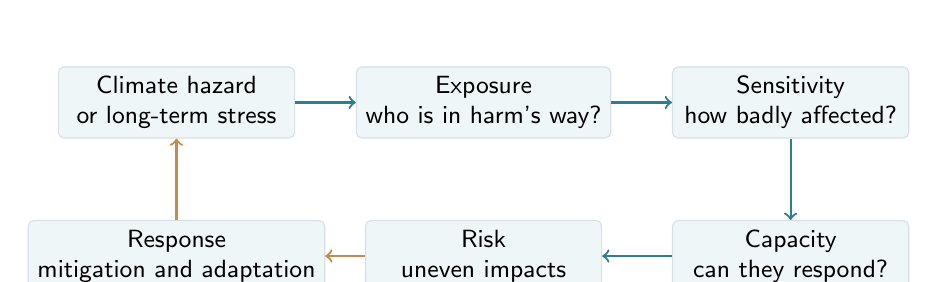
\begin{tikzpicture}[node distance=1.6cm, every node/.style={font=\sffamily\small}]
  \tikzstyle{box}=[rectangle, rounded corners=2pt, draw=RuleGray, fill=SoftBlue,
  minimum width=3.0cm, minimum height=0.82cm, align=center]
  \node[box] (hazard) {Climate hazard\\or long-term stress};
  \node[box, right of=hazard, xshift=2.3cm] (exposure) {Exposure\\who is in harm's way?};
  \node[box, right of=exposure, xshift=2.3cm] (sensitivity) {Sensitivity\\how badly affected?};
  \node[box, below of=sensitivity, yshift=-0.35cm] (capacity) {Capacity\\can they respond?};
  \node[box, left of=capacity, xshift=-2.3cm] (risk) {Risk\\uneven impacts};
  \node[box, left of=risk, xshift=-2.3cm] (response) {Response\\mitigation and adaptation};
  \draw[->, thick, color=AccentTeal] (hazard) -- (exposure);
  \draw[->, thick, color=AccentTeal] (exposure) -- (sensitivity);
  \draw[->, thick, color=AccentTeal] (sensitivity) -- (capacity);
  \draw[->, thick, color=AccentTeal] (capacity) -- (risk);
  \draw[->, thick, color=AccentGold] (risk) -- (response);
  \draw[->, thick, color=AccentGold] (response) -- (hazard);
\end{tikzpicture}
\end{center}

\section{25-Minute Practice Block}

Use the workbook file
\term{2026-04-30-food-health-essay-planning-workbook.pdf}. The plan asks you
to choose one Food and health Paper 1 extended-answer prompt from a choice of
two and underline where evaluation happens.

\subsection{Choice Of Two Prompts}

\boxnote{SoftTint}{Prompt A.}{\exam{Evaluate} the role of stakeholders in
improving food security and health in one or more places.}

\vspace{0.5em}

\boxnote{SoftBlue}{Prompt B.}{\exam{To what extent} can sustainable food
systems reduce health inequalities?}

\subsection{The 25-Minute Rhythm}

\rowcolors{2}{TableStripe}{white}
\begin{tabularx}{\textwidth}{L{0.15\textwidth}Y Y}
\toprule
\textbf{Time} & \textbf{Task} & \textbf{Output} \\
\midrule
0--3 min & Closed-book recall of stakeholders, food-security dimensions, and
health inequality factors & Fast idea bank \\
3--6 min & Choose Prompt A or B and unpack command term & One focused question
translation \\
6--10 min & Decide judgment and criteria & One thesis sentence \\
10--18 min & Plan three main paragraphs & Evidence, explanation, and one
underlined evaluation phrase per paragraph \\
18--22 min & Write conclusion in note form & Final judgment with degree of
success or extent \\
22--25 min & Self-check and strengthen evaluation & One improved underlined
sentence \\
\bottomrule
\end{tabularx}
\rowcolors{2}{}{}

\subsection{End-Of-Day Output}

You are finished with April 30 if you have:

\begin{itemize}
  \item chosen one of the two Food and health extended-answer prompts
  \item written a thesis with a clear judgment
  \item planned at least three paragraphs with evidence, explanation, and
  evaluation
  \item underlined the exact places where evaluation happens
  \item used Brazil and Nestle or another class-specific Food and health case
  accurately
  \item explained health inequality with at least three causal factors
  \item defined vulnerability, resilience, mitigation, and adaptation from
  memory
  \item logged one Food and health case-study detail and one Climate case-study
  detail to fill on May 1
\end{itemize}

\boxnote{SoftGreen}{Carry forward.}{On Friday 2026-05-01, the plan becomes
case-study bank day. Bring forward today's gaps using the format:
\term{place} $\rightarrow$ \term{issue} $\rightarrow$ \term{causes}
$\rightarrow$ \term{impacts} $\rightarrow$ \term{response} $\rightarrow$
\term{evaluation}.}

\end{document}
